\documentclass[12pt]{article}

% This first part of the file is called the PREAMBLE. It includes
% customizations and command definitions. The preamble is everything
% between \documentclass and \begin{document}.

\usepackage[margin=1in]{geometry}  % set the margins to 1in on all sides
\usepackage{graphicx}              % to include figures
\usepackage{amsmath}               % great math stuff
\usepackage{amsfonts}              % for blackboard bold, etc
\usepackage{amsthm}                % better theorem environments
\usepackage{amssymb} 
\usepackage{mathptmx}
\usepackage{graphicx}
\usepackage{enumerate}
\usepackage{listings}
\usepackage{xcolor}
\usepackage{array}

% various theorems, numbered by section

\newtheorem{thm}{Theorem}[section]
\newtheorem{lem}[thm]{Lemma}
\newtheorem{prop}[thm]{Proposition}
\newtheorem{cor}[thm]{Corollary}
\newtheorem{conj}[thm]{Conjecture}
\newtheorem{mydef}[thm]{Definition}


\lstset{
	basicstyle          =   \sffamily,          
	keywordstyle        =   \bfseries,          
	commentstyle        =   \rmfamily\itshape,  
	stringstyle         =   \ttfamily,  
	flexiblecolumns,                
	numbers             =   left,   
	showspaces          =   false,  
	numberstyle         =   \fontsize{5}{skip},    
	showstringspaces    =   false,
	captionpos          =   t,      
	frame               =   lrtb,   
}

\lstdefinestyle{cpp}{
	language        =   cpp, 
	basicstyle      =   \fontsize{5}{skip},
	numberstyle     =   \fontsize{5}{skip},
	keywordstyle    =   \color{blue},
	keywordstyle    =   [2] \color{teal},
	stringstyle     =   \color{magenta},
	commentstyle    =   \color{red}\ttfamily,
	breaklines      =   true,   
	columns         =   fixed,  
	basewidth       =   0.5em,
}
\begin{document}


\title{ CSE 102 Spring 2021\\
	Extra Credit Problem}

\author{Jaden Liu \\ 
University of California at Santa Cruz\\
Santa Cruz, CA 95064 USA }

\maketitle


\section{Extra Credit Problem} 
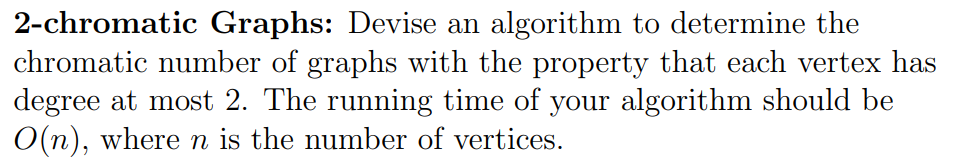
\includegraphics[scale=0.4]{1.png}
\begin{proof}
	Assume we have the worst situation that each vertex has 2 degree. We first initialize a empty hash table to save the vertex that we have examined. We first pick any vertex as the the initial point, adding it to the hash table and giving it a color. Then we can define the two edges as the "left" and "right". So we first start with the left branch. Then the sub-node will also have two branch, one connecting the father node and one connecting the other node. The color of the sub-node is determined by both the father color and the other node. We can list all the situations:
	
	a): The other node is not in the hash table. We just need to pick a color that different from the father node and adding the sub-node to the hash table.
	
	b): The other node is in the hash table, then we have 2 cases:
	
	1. The other node has the same color with the sub-node, then we need to change the sub-node's color to a third color that is different from both the other node and the parent node.
	
	2.The other node has the different color with the sub-node, then we can just easily use the same old two types color alternately. We do not need to use a third type of color.\\
	After adding the sub-node and its color into the hash table, then we make the sub-node to a new father node and continue this recursion until the size of the hash table reaches $n$.\\
	Since the time complexity of looking up hash table is $O(1)$, and we only need to examine each node once, the total time should be $O(n)$.
\end{proof}
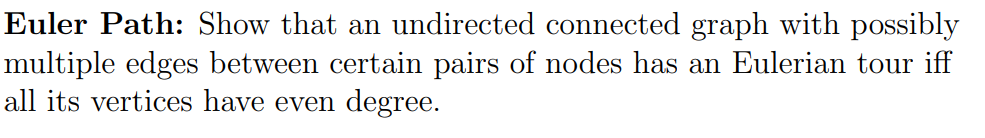
\includegraphics[scale=0.4]{2.png}
\begin{proof}
	1. Necassary: If the graph has an Eulerian tour, each vertex has a even degree.
	
	Suppose $G$ is an Euler diagram, then G is obviously connected. If the graph has a Eulerian tour, then when we run this route on each vertex, we must have two edges, which are "in" and "out". That means, we have a previous vertex who leads to this vertex and this vertex must leads to another vertex. Since the definition of the Eulerian tour, these two vertex must be different from previous. Thus, the degree of each vertex must increase as a multiples of 2, which is even in the end.\\
	2. Sufficient: If each vertex has even degree, we need to prove this graph has a Eulerian tour.
	
	We can prove by induction. Assume we have a graph $G$ and $m$ is the number of edges. \\
	Base Case: m=1\\
	This is trivial that the graph will only has one edge which is connect to itself. Thus it generate a Eulerian tour.\\
	Induction step: Assume that a connected graph with less than $m$ edges must be an Euler graph when the vertex degree is even. Now consider a graph G with $m$ edges, we need to prove it has Eulerian path. Since each vertex has an even degree, we can always leave the node after entering it. When the route returns to the starting point, it draws a closed path, denoted as $H$. Delete all the edges of H from the graph $G$. The resulting graph is denoted as $G'$. $G'$ may not be connected, but the degree of each vertex is still even. Consider the connected components of G. Since they are all connected, the vertex degrees are all even, and the number of edges are all less than $m$, so according to the induction hypothesis, they are all Euler graphs. In addition, since $G$ is connected, they all share one or several common vertices with H, so they together form a closed path. This means that G is an Euler diagram.
	
\end{proof}

\end{document}
